\documentclass[
	% -- opções da classe memoir --
	12pt,				% tamanho da fonte
	%openright,			% capítulos começam em pág ímpar (insere página vazia caso preciso)
	oneside,			% para impressão em verso e anverso. Oposto a oneside
	a4paper,			% tamanho do papel. 
	% -- opções da classe abntex2 --
	%chapter=TITLE,		% títulos de capítulos convertidos em letras maiúsculas
	%section=TITLE,		% títulos de seções convertidos em letras maiúsculas
	%subsection=TITLE,	% títulos de subseções convertidos em letras maiúsculas
	%subsubsection=TITLE,% títulos de subsubseções convertidos em letras maiúsculas
	% -- opções do pacote babel --
	english,			% idioma adicional para hifenização
	brazil				% o último idioma é o principal do documento
]{abntex2}

% ---
% Pacotes básicos 
% ---
\usepackage{lmodern}				% Usa a fonte Latin Modern			
\usepackage[T1]{fontenc}			% Selecao de codigos de fonte.
\usepackage[utf8]{inputenc}		% Codificacao do documento (conversão automática dos acentos)
\usepackage{lastpage}			% Usado pela Ficha catalográfica
\usepackage{indentfirst}			% Indenta o primeiro parágrafo de cada seção.
\usepackage{color}				% Controle das cores
\usepackage{graphicx}			% Inclusão de gráficos
\usepackage{microtype}			% para melhorias de justificação
\usepackage{multirow}			% mesclar linhas em tabelas
\usepackage{comment}				% habilita comentário em bloco

% ---
% Pacotes de citações
% ---
%\usepackage[brazilian,hyperpageref]{backref}		% Paginas com as citações na bibl
\usepackage[alf]{abntex2cite}					% Citações padrão ABNT

% --- 
% CONFIGURAÇÕES DE PACOTES
% --- 
% Configurações do pacote backref
% Usado sem a opção hyperpageref de backref
%\renewcommand{\backrefpagesname}{Citado na(s) página(s):~}
% Texto padrão antes do número das páginas
%\renewcommand{\backref}{}
% Define os textos da citação
%\renewcommand*{\backrefalt}[4]{
%	\ifcase #1 %
%		Nenhuma citação no texto.%
%	\or
%		Citado na página #2.%
%	\else
%		Citado #1 vezes nas páginas #2.%
%	\fi}%

% ---
% Informações de dados para CAPA e FOLHA DE ROSTO
% ---
\titulo{Proposta de melhoria de desempenho do SIGA utilizando NGINX como servidor HTTP}
\autor{Lucas Rafael Araujo Andrade}
\local{Diamantina}
\data{Dezembro de 2014}
\orientador{Alexandre Ramos Fonseca}
\instituicao{%
  Universidade Federal dos Vales do Jequitinhonha e Mucuri - UFVJM
  \par
  Faculdade de Ciências Exatas e Tecnológicas - FACET
  \par
  Departamento de Computação - DECOM
  \par
  Bacharelado em Sistemas de Informação}
\tipotrabalho{Trabalho de Conclusão de Curso de Gradua}
% O preambulo deve conter o tipo do trabalho, o objetivo, 
% o nome da instituição e a área de concentração 
\preambulo{Trabalho de conclusão de curso apresentado à banca examinadora
 Designada pelo Colegiado do Curso de Sistemas de Informação como parte
 dos requisitos da disciplina de Projeto Orientado II para
 obtenção do grau de Bacharel em Sistemas de Informação.}
% ---


% ---
% Configurações de aparência do PDF final

% informações do PDF
\makeatletter
\hypersetup{
     	%pagebackref=true,
		pdftitle={\@title}, 
		pdfauthor={\@author},
    		pdfsubject={\imprimirpreambulo},
	    pdfcreator={LaTeX with abnTeX2},
		pdfkeywords={NGINX}{APACHE2}{SIGA}{UFVJM}{Monografia}, 
		colorlinks=false,       		% false: boxed links; true: colored links
    		%linkcolor=blue,          	% color of internal links
    		%citecolor=blue,        		% color of links to bibliography
    		filecolor=magenta,      		% color of file links
		%urlcolor=blue,
		bookmarksdepth=4,
		pdfborder = {0 0 0}
}
\makeatother

% --- 
% Espaçamentos entre linhas e parágrafos 
% --- 
% O tamanho do parágrafo é dado por:
\setlength{\parindent}{1.3cm}
% Controle do espaçamento entre um parágrafo e outro:
\setlength{\parskip}{0.2cm}  % tente também \onelineskip

% ---
% compila o indice
% ---
\makeindex

% ----
% Início do documento
% ----
\begin{document}

% Retira espaço extra obsoleto entre as frases.
\frenchspacing 

% ----------------------------------------------------------
% ELEMENTOS PRÉ-TEXTUAIS
% ----------------------------------------------------------
\pretextual

% ---
% Capa
% ---
\imprimircapa

% ---
% Folha de rosto
% ---
\imprimirfolhaderosto

% ---
% Inserir folha de aprovação
% ---
\begin{folhadeaprovacao}

  \begin{center}
    {\ABNTEXchapterfont\large\imprimirautor}

    \vspace*{\fill}\vspace*{\fill}
    \begin{center}
      \ABNTEXchapterfont\bfseries\Large\imprimirtitulo
    \end{center}
    \vspace*{\fill}
    
    \hspace{.45\textwidth}
    \begin{minipage}{.5\textwidth}
        \imprimirpreambulo
    \end{minipage}%
    \vspace*{\fill}
   \end{center}
        
   APROVADO em:        /        /

 
   \assinatura{\textbf{Professor Me. Áthila Rocha Trindade} \\ Universidade Federal dos Vales do Jequitinhonha e Mucuri}
   \assinatura{\textbf{Professor Me. Eduardo Pelli} \\ Universidade Federal dos Vales do Jequitinhonha e Mucuri}
   \assinatura{\textbf{\imprimirorientador} \\ Orientador}
      
   \begin{center}
    \vspace*{0.5cm}
    {\large\imprimirlocal}
    \par
    {\large\imprimirdata}
    \vspace*{1cm}
  \end{center}
  
\end{folhadeaprovacao}

% ---
% Dedicatória
% ---
\begin{dedicatoria}
   \vspace*{\fill}
   \centering
   \noindent
   \textit{Dedico esse trabalho à mulher que tornou isso tudo possível. Te Amo Mãe!} \vspace*{\fill}
\end{dedicatoria}

% ---
% Agradecimentos
% ---
\begin{agradecimentos}

Agradeço primeiramente aos meus mestres que em todos esses anos se empenharam 
em passar o máximo de conhecimento possível, em especial o meu orientador 
Alexandre pela oportunidade de desenvolver esse projeto.

Agradeço aos meus amigos de Bocaiuva e Diamantina: Diego, Hebert, Mayra, 
Natália, Fernanda, Lorena e Paulo Barreto. Saibam que todos, de alguma forma, 
fizeram diferença na minha vida e com todos vocês eu aprendi algo.

Agradeço especialmente aos meus grandes amigos Arthur, Leandro e Thalita, por 
todas as conversas de bar, trabalhos, shows e tardes e mais tardes escutando 
música, jogando conversa fora e nos divertindo. Vocês fizeram uma diferença 
enorme na minha vida e eu devo muito a todos vocês!

Agradeço as minhas amigas de Winnipeg: Tamara, Carol, Stefanie, Juliana e 
Ingrid. Com vocês por perto tudo se tornou menos difícil e mais alegre durante 
a minha estadia no Canadá.

Agradeço a Lili pelo apoio durante os mais de dois anos em que estivemos 
juntos. Saiba você que teve um papel muito importante na minha vida e lembrarei 
sempre dos nossos momentos juntos pro resto da minha vida.

Agradeço aos meus familiares que diretamente ou indiretamente me ajudaram 
durante todos esses anos de Diamantina: Tio Vendoval, Tia Letícia (\textit{In 
Memorian}), Vó Nita e Tio Antônio.

Agradeço aos Técnicos-Administrativos do DTI da UFVJM: Everton, William, 
Marcelo, Rodrigo, André e Ricardo Brasil, por todo o conhecimento e experiência 
compartilhados com nós, estagiários.

E por último, porém mais importante, a mulher que por todos os meus 26 anos de 
vida me aturou com um amor incondicional que somente uma Mãe é capaz de sentir. 
Saiba, Mãe, que sem você, nada disso seria possível. Te amo incondicionalmente 
também!

\end{agradecimentos}

% ---
% Epígrafe
% ---
\begin{epigrafe}
    \vspace*{\fill}
	\begin{flushright}
		\textit{``Code is Poetry\\
		(Wordpress.org)}
	\end{flushright}
\end{epigrafe}

% ---
% Resummo
% ---
\setlength{\absparsep}{18pt} % ajusta o espaçamento dos parágrafos do resumo
\begin{resumo}
O presente trabalho tem por objetivo identificar o grau de eficiência do 
servidor HTTP Nginx, para processamento das requisições recebidas, em 
comparação ao servidor Apache HTTP Server, atualmente utilizado pela 
Universidade Federal dos Vales do Jequitinhonha e Mucuri – UFVJM em seu Sistema 
Integrado de Gestão Acadêmica - SIGA. Ambos os servidores em estudo estão entre 
os sete mais utilizados no mundo e entre os cinco mais utilizados pelos sítios 
mais acessados mundialmente. Os dados foram coletados após realização de testes 
de desempenho com o uso da ferramenta ApacheBench, instalada em duas máquinas 
virtuais, igualmente configuradas e instaladas através do software de 
virtualização VirtualBox, hospedadas em computador portátil.\\
Com base em levantamento do número de usuários da comunidade acadêmica da 
UFVJM, foram definidos quinze valores de testes, quatro cenários  de acesso 
simultâneo e seis métricas indicadoras de eficiência. A fim de permitir uma 
melhor visualização dos resultados obtidos e análise, os dados gerados foram 
dispostos em três gráficos divididos em três faixas de valores e um gráfico com 
a quantidade total de requisições testadas. A análise dos resultados foi 
realizada para cada métrica, de modo individualizado, explicitando a média de 
desempenho de cada servidor. Após análise é exposta a conclusão acerca da 
eficiência demonstrada por pelo servidor HTTP Nginx e Apache HTTP Server e 
parecer sobre  qual servidor se mostra  mais adequado e eficiente ao SIGA.


 \textbf{Palavras-chaves}: Apache. Nginx. SIGA. UFVJM.
\end{resumo}

% ---
% Abstract
% ---
\begin{resumo}[Abstract]
 \begin{otherlanguage*}{english}
The goal of this work is to identify the Nginx HTTP server efficiency, for 
processing requisitions compared to the Apache HTTP server, currently in use by 
the Federal University of the Vales of Jequitinhonha and Mucuri – UFVJM in its 
Academic Integrated Management System - SIGA. Both server studied are among the 
seven most used in the world and among the five most used by the most accessed 
web sites wide world. The data has been collected after performance tests 
performed with the ApacheBench tool, installed in two virtual machines, equally 
configured and installed in the visualization software VirtualBox hosted in a 
portable computer.\\
Based on the amount of users in the academic community oh the UFVJM, was 
defined fifteen tests values, four simultaneous access scenarios and six 
efficiency metrics. In order to provide a better visualization of the results 
acquired, the collected data was distributed in tree graphs divided in tree 
ranges of values an a graph with the total amount of requisitions tested. The 
result analysis was made for each metric in an individual way, showing the 
average performance from each server. After the analysis, the conclusion about 
the Nginx and Apache HTTP server is shown and concludes about which server is 
more adequate e efficient to SIGA.
   \vspace{\onelineskip}
 
   \noindent 
   \textbf{Key-words}: Apache. Nginx. SIGA. UFVJM.
 \end{otherlanguage*}
\end{resumo}

% ---
% Lista de Figuras
% ---
\pdfbookmark[0]{\listfigurename}{lof}
\listoffigures*
\cleardoublepage

% ---
% Lista de Tabelas
% ---
\pdfbookmark[0]{\listtablename}{lot}
\listoftables*
\cleardoublepage

% ---
% Siglas e Abreviaturas
% ---
\begin{siglas}
  \item[API] \textit{Application Programming Interface}
  \item[CGI] \textit{Common Gateway Interface}
  \item[CSS] \textit{Cascading Style Sheets}
  \item[IP] \textit{Internet Protocol}
  \item[HTML] \textit{Hypertext Markup Language}
  \item[HTTP] \textit{Hipertext Transport Protocol}
  \item[ODBC] \textit{Open Database Connection}
  \item[PDF] \textit{Portable Document Format}
  \item[PDI] Plano de Desenvolvimento Institucional
  \item[PDO] \textit{PHP Data Object}
  \item[PHP] \textit{Hypertext Preprocessor}
  \item[PHP-FPM] \textit{PHP FastCGI Process Manager}
  \item[SIGA] Sistema Integrado de Gestão Acadêmica
  \item[SGBD] Sistema de Gerenciamento de Banco de Dados
  \item[TCP] \textit{Transmission Control Protocol}
  \item[TCP/IP] \textit{Transmission Control Protocol/Internet Protocol	}
  \item[URI] \textit{Uniform Resource Identifier}
  \item[URL] \textit{Uniform Resource Locator}
  \item[UFVJM] Universidade Federal dos Vales do Jequitinhonha e Mucuri
  \item[W3C] \textit{World Wide Web Consortium}
  \item[WWW] \textit{World Wide Web}
  \item[XML] \textit{Extensible Markup Language}
  \item[XHTML] \textit{Extensible Hypertext Markup Language}
\end{siglas}

% ---
% Sumário
% ---
\pdfbookmark[0]{\contentsname}{toc}
\tableofcontents*
\cleardoublepage

% ----------------------------------------------------------
% ELEMENTOS TEXTUAIS
% ----------------------------------------------------------
\textual

% ---
% Introducao
% ---
\chapter{Introdução}\label{cap:introducao}
Com o avanço dos computadores e das redes de comunicação, os sistemas de 
informação foram sendo transferidos dos computadores pessoais para os 
servidores \textit{web}, de onde eles podem ser acessados, virtualmente, a 
partir de todo o mundo. Para que esses sistemas funcionem, eles precisam de 
\textit{softwares} que atendam as requisições que chegam ao servidor a partir 
da rede de computadores usando o protocolo HTTP. Esses softwares são chamados 
servidores HTTP.\\
O aumento do uso de sistemas baseados na \textit{web} por organizações criou a 
necessidade de desenvolver aplicações que geram conteúdo dinamicamente. São 
essas aplicações que permitem às organizações entregarem produtos, serviços e 
mensagens cujas formas e conteúdos são, em parte, determinadas pelas 
necessidades do usuário.\\
Este movimento para se afastar de conteúdos estáticos está levando ao limite e 
expões as fragilidades dos ambientes onde essas aplicações são 
executadas. Mais importante, esses ambientes não oferecem o desempenho que 
essas aplicações exigem. É preciso uma nova infraestrutura de comunicação para 
conectar servidores \textit{web} com essas novas aplicações.\\
De acordo com \citeonline{bondi2000}, escalabilidade é um atributo desejável de 
uma rede, sistema ou processo. O conceito tem a ver com a habilidade do sistema 
em acomodar uma quantidade sempre maior de elementos ou objetos, de processar 
uma quantidade crescente de trabalho de forma fácil e ou ser suscetível a 
ampliação. Quando se está desenvolvimento um sistema, deseja-se que 
ele seja escalável.\\
Quando se diz que um sistema não é escalável (ou que ele não escala), damos a 
entender que o custo adicional de lidar com o aumento em trafego ou tamanho é 
excessivo, ou que o sistema não consegue lidar com esse nível elevado de 
acesso. O custo pode ser quantificado de várias formas, incluído, porém não 
limitado à tempo de resposta, uso de processamento, espaço, memória ou até 
mesmo dinheiro. Um sistema que não escala bem, adiciona custos de manutenção ou 
danifica a qualidade do serviço, pode atrasar ou privar o usuário de 
oportunidades de lucro e, eventualmente, precisará ser substituído.\\
A escalabilidade de um sistema sujeito a expansão é crucial para o seu 
sucesso a longo prazo. Ao mesmo tempo, o conceito de escalabilidade e o 
entendimento dos fatores que aumenta ou diminui são vagos e até mesmo 
subjetivos. Desenvolvedores de sistemas e analistas de desempenho têm um 
sentimento intuitivo sobre escalabilidade, pois os fatores determinantes não 
são claros e podem variar de um sistema para outro.\\
A escalabilidade de um sistema pode ser comprometida por desperdícios herdados 
de ações repetidas de forma frequente, pela presença de algoritmos de acesso 
que levam a \textit{deadlock} ou que resultam em um escalonamento ruim de 
recursos. Tais sistemas podem funcionar bem quando a carga está baixa, mas 
sofrer uma degradação substancial de desempenho quando a carga aumenta.\\
Atualmente, a UFVJM, utiliza o SIGA – Sistema Integrado de Gestão Acadêmica, 
adquirido da Universidade Federal de Juiz de Fora em 2007. O sistema é 
desenvolvido na linguagem de programação PHP com o apoio do \textit{framework} 
Miolo e utiliza o Apache HTTP \textit{Server} como servidor HTTP e o PostgreSQL 
como SGBD.\\
O Apache, desde 1.995 tem sido o servidor HTTP mais utilizado no mundo. Em 
Outubro de 2.014, de acordo com pesquisa realizada em 1.028.932.208 de sítios 
pela empresa Netcraft, o Apache era usado por 37,79\% (385.354.994) desses 
sítios, com o Microsoft IIS aparecendo em segundo com 33,58\% (345.485.419) e o 
Nginx em terceiro com 14,42\% (148.330.190) de participação nos sítios, como 
visto na figura \ref{fig:webservers-utilizacao}.\\
Nessa mesma pesquisa, realizada com base em um milhão dos sites mais acessados 
no mundo, o Apache é apontado como o servidor mais utilizado por 50,19\% 
(501,922) destes, sendo o Nginx apontado em segundo lugar com 14,36\% 
(25,588,943), conforme a figura \ref{fig:webservers-utilizacao-milhao}\\.
\begin{figure}[htb]
	\centering
	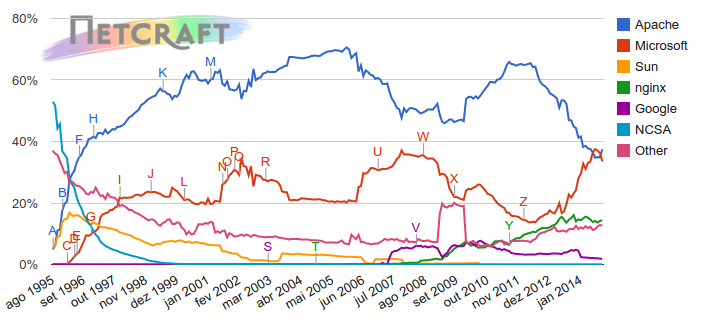
\includegraphics[width=1\linewidth]{figuras/grafico1}
	\caption{Utilização de Servidores \textit{web} no mundo.}
	\label{fig:webservers-utilizacao}
\end{figure}

\begin{figure}[htb]
	\centering
	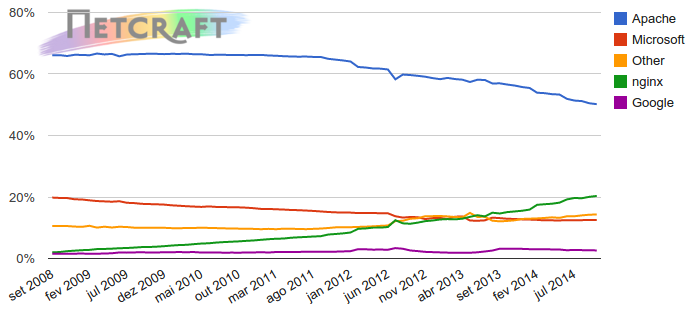
\includegraphics[width=1\linewidth]{figuras/grafico2} 
	\caption{Utilização de Servidores \textit{web} entre os 1.000.000 de sítios 
	mais acessados no mundo.}
	\label{fig:webservers-utilizacao-milhao}
\end{figure}
Analisando os gráficos presentes nas figuras \ref{fig:webservers-utilizacao} e 
\ref{fig:webservers-utilizacao-milhao}, é possível notar uma queda na 
utilização do Apache em detrimento de outros servidores HTTP, sendo mais 
notória a queda na utilização entre 1 milhão de sítios mais acessados. É 
possível notar também o aumento no uso do Nginx, principalmente entre os 1 
milhão de sítios mais acessados no mundo. É necessário frisar que só porque uma 
tecnologia está em ascensão, não significa que ela é melhor, mas sim é 
necessário investigar os motivos pelo qual a tecnologia está crescendo em 
número de utilizadores.\\
Tendo sido desenvolvidos em épocas diferentes, o Apache e o Nginx trabalham de 
forma diferente na hora de atender as requisições HTTP que chegam ao servidor.\\
De acordo com \citeonline{rowe}, o Apache cria processos e \textit{threads} 
para lidar com as requisições, ficando a cargo do administrador do servidor a 
tarefa de configurar o Apache para controlar o numero máximo de processos e 
\textit{threads} permitidos. Muitas \textit{threads} podem exaurir a memória 
principal(RAM) e pode forçar o servidor a usar memória \textit{SWAP}, 
degradando severamente o desempenho. Além disso, quando chega ao limite de 
processos, o Apache passa a recusar conexões.
\section{Motivação}
De acordo com o Plano de Desenvolvimento Institucional para o ciclo 2.012 - 
2.016 da UFVJM, além dos quatro \textit{campi} já implantados (Diamantina, 
Teófilo Otoni, Janaúba e Unaí) o existe o projeto para a implantação de outros 
quatro \textit{campi} universitários nas cidade de Capelinha, Araçuaí, Almenara 
e Nanuque, totalizando oito \textit{campi} espalhados pelas regiões Norte, 
Noroeste, Vales do Jequitinhonha e Mucuri do estado de Minas Gerais. O 
PDI contempla também a ampliação da oferta de vagas para cursos de graduação 
nos \textit{campi} Diamantina e Teófilo Otoni. Com a expansão das Universidades 
Federais através do programa REUNI, por ano são admitidos 3500 alunos de 
graduação, pós-graduação e educação à distância além de novos servidores 
técnicos-administrativos e professores. Somente no último edital para seleção 
de técnicos-administrativos, foram oferecias 148 vagas.\\
Em julho de 2.014, data do último levantamento, a Universidade Federal dos 
Vales do Jequitinhonha e Mucuri tinha 8.121 alunos, 576 professores e 421 
servidores técnicos-administrativos, espalhados em quatro \textit{campi} 
universitários, fazendas experimentais e pólos de ensino em educação à 
distância, totalizando 9.118 pessoas que interagem com a universidade 
diariamente.\\
Em épocas de pico de utilização do SIGA, as reclamações de lentidão e problemas 
no sistemas são frequentes, as vezes impossibilitando a utilização do mesmo. Os 
picos mais notório são: fim de período letivo da graduação, quando alunos e 
professores acessam o sistema para olhar e lançar notas, respectivamente; e 
rematricula dos alunos da graduação, quando os mesmos escolhem as matérias que 
desejam cursar no período seguinte.\\




No ano de 2.014, blablabla






Com o crescente aumento de alunos, servidores públicos (professores e 
técnicos-administrativos) e teceirizados na universidade, a tendência é que a 
utilização do SIGA se torne mais problemática.
Com isso em mente, a utilização do servidor HTTP Nginx pode ajudar a amenizar 
os problema de desempenho do SIGA.\\
\section{Objetivos}
Identificar se a utilização do servidor HTTP Nginx é mais eficiente do que o 
utilizado atualmente, o Apache HTTP \textit{Server}.\\
\section{Objetivos específicos}
Analisar os dados coletados a partir de testes realizados para identificar se o 
Nginx é mais eficiente do que o Apache; apresentar a solução encontrada e 
analisar o que pode ser feito para evitar a substituição ou reconstrução do 
SIGA.\\
\section{Organização do trabalho}
O trabalho está organizado em oito capítulos, sendo essa introdução o primeiro. 
O capítulo \ref{cap:fundamentacao-teorica}, será exposto toda a teoria por trás 
do estudo feito. No capítulo \ref{cap:tecnologias_utilizadas}, serão descritos 
os programas e ferramentas utilizados implicitamente e explicitamente nos 
testes. No capítulo \ref{cap:metodologia} será descrito como os testes foram 
realizados e quais dados foram coletados e descrever os ambientes onde foram 
feitos os teste de desempenho do Apache e do Nginx. No capítulo 
\ref{cap:analise-dos-dados} os dados serão apresentados e 
será feita uma análise sobre o desempenho dos dois servidores HTTP. E 
finalmente, no capítulo \ref{cap:conclusao} eu apresentarei as minhas 
conclusões sobre o estudo.\\


% ---
% Fundamentacoes Teoricas
% ---
\chapter{Fundamentação Teórica}\label{cap:fundamentacao-teorica}

Este capítulo se destina a apresentar alguns conceitos teóricos para o 
entendimento da proposta desse estudo.

\section{Aplicação cliente/servidor}

Para entender o que é uma aplicação cliente/servidor, é preciso primeiramente 
definir o que é cliente e servidor.

\subsection{Cliente}
Cliente é:

\begin{citacao}
Um solicitante de informações em rede, normalmente um computador ou estação de 
trabalho, que pode consultar o banco de dados e/ou outras informações de um 
servidor. \cite{stallings2005}
\end{citacao}

Ainda de acordo com \citeonline{stallings2005}, o cliente é um computador ou 
estação de trabalho, que apresenta ao usuário final uma interface gráfica de 
alto nível e amigável, incluindo o uso de janelas e \textit{mouse}. 

\subsection{Servidor}

Servidor é:

\begin{citacao}
	
Um computador, normalmente uma estação de trabalho poderosa ou um 
\textit{mainframe} que abriga informações para manipulação por clientes em 
rede. \cite{stallings2005}

\end{citacao}

Ainda de acordo com \citeonline{stallings2005}, cada servidor no ambiente 
cliente/servidor fornece um conjunto de serviços compartilhados.

\subsection{Aplicações cliente/servidor}

As aplicações cliente/servidor são um conjunto de programas que funcionam no 
computador cliente, ou seja, aquele que esta solicitando um recurso pela rede, 
e no computador servidor, aquele que provê o recurso solicitado. As 
solicitações de recursos ou informações partem do programa instalado no 
computador do usuário (cliente), trafegam por uma rede de computadores, 
geralmente utilizando o protocolo de comunicação HTTP até o servidor 
responsável por prover o recurso ou informação solicitado pelo programa do 
cliente.

As aplicações cliente/servidor são muito utilizadas na construção de sistemas 
de informação, onde os dados armazenados pelos servidores precisam estar 
disponíveis para os usuários do sistema. É também o principal modelo utilizado 
em sistemas de informação baseados na \textit{web}, onde o cliente acessa o 
sistema através de um navegador \textit{web}.

\section{Protocolo de comunicação}

De acordo com \citeonline{stallings2005}, protocolo pode ser entendido como uma 
convenção que controla e possibilita uma conexão, comunicação e transferência 
de dados entre dois sistemas computacionais. De maneira simples, protocolos 
podem ser definidos como as regras que governam a sintaxe, semântica e 
sincronização da comunicação. 
De acordo com \citeonline{stallings2005}, um protocolo é usado para a 
comunicação entre entidades em sistemas diferentes. Para que entidades 
diferentes se comuniquem com facilidade, elas precisam adotar uma ``língua'' em 
comum. O quê e como é comunicado, deve estar de acordo com as convenções 
combinadas entre as entidades envolvidas. Essas convenções são denominadas 
protocolos, que são conjuntos de regras para controlar a troca de 
dados entre entidades. Os principais elementos de um protocolo são:

\begin{itemize}
	\item Sintaxe: Inclui elementos como formato de dados e níveis de sinal;
	\item Semântica: Inclui informações de controle para coordenação e 
	tratamento de erro;
	\item Temporização: Inclui combinação de velocidade e sequência.
\end{itemize}

\section{Modelo TCP/IP}

O TCP/IP (\textit{Transmission Control Protocol/Internet Protocol}), é um 
conjunto de protocolos, resultante de pesquisas e desenvolvimentos realizados 
pela ARPANET (\textit{Advanced Research Project Agency Network}) e financiada 
pela DARPA (\textit{Defense Advanced Research Projects Agency}), agência de 
pesquisa militar do governo dos Estados Unidos, e que hoje são utilizados como 
padrões de comunicação na Internet.

Ao contrário do modelo OSI(Open Systems Interconnections), o TCP/IP não pode 
ser considerado um modelo e sim um conjunto de protocolos. Esse protocolos, 
assim como no modelo OSI, podem ser organizados em camadas relativamente 
independentes, com a diferença de que no modelo OSI existem sete camadas e no 
TPC/IP existem cinco. As camadas do TCP/IP são:

\begin{itemize}
	\item Camada de aplicação
	\item Camada de transporte
	\item Camada de rede
	\item Camada de enlace
	\item Camada física
\end{itemize}

Para efeito de comparação, as camadas do modelo OSI são:

\begin{itemize}
	\item Camada de aplicação
	\item Camada de apresentação
	\item Camada de sessão
	\item Camada de transporte
	\item Camada de rede
	\item Camada de enlace
	\item Camada física
\end{itemize}

%aplicação
\subsection{Camada de aplicação}

De acordo com \citeonline{stallings2005}, a camada de aplicação é utilizada 
pela maioria dos programas para se comunicar através de uma rede com outros 
programas. Processos que 
funcionam nessa camada são específicos da aplicação; o dado é passado do 
programa de rede, no formato usado internamente por essa aplicação, e é 
codificado dentro do padrão de um protocolo. Os protocolos mais comuns são:

\begin{itemize}
	\item SMTP (\textit{Simple Mail Transport Protocol}): é utilizado para a 
	comunicação entre serviços de correio eletrônico na Internet.
	\item POP (\textit{Post Office Protocol}): é utilizado para recuperação de 
	mensagens de correio eletrônico via Internet.
	\item IMAP (\textit{Internet Mail Access Protocol}): é utilizado para 
	recuperação de mensagens de correio eletrônico via Internet, mais 
	avançado que o POP.
	\item HTTP (\textit{Hypertext Transport Protocol}): utilizado para a 
	publicação de sites \textit{web} na Internet.
	\item FTP (\textit{File Transfer Protocol}): utilizado para publicação e 
	transferência de arquivos via Internet.

\end{itemize}

%host a host
\subsection{Camada de transporte}

A camada de transporte (ou \textit{host} a \textit{host}), de acordo com 
\citeonline{stallings2005}, é responsável pela 
transferência eficiente, confiável e econômica dos dados entre o computador de 
origem e de destino, independente do tipo, topologia ou configuração das redes 
físicas existentes entre elas, garantindo ainda que os dados cheguem sem erros 
e na sequência correta.

A camada de transporte é uma camada fim-a-fim, isto é, uma entidade desta 
camada só se comunica com a sua entidade semelhante do destinatário. A camada 
de transporte provê mecanismos que possibilitam a troca de dados fim-a-fim, não 
possibilitando, assim, a comunicação com entidades intermediárias. A camada 
possui dois protocolos: o UDP (\textit{User Datagram Protocol}) e o TCP 
(\textit{Transmission Control Protocol}).

O protocolo UDP realiza apenas a multiplexação para que várias aplicações 
possam acessar o sistema de comunicação de forma coerente. O protocolo TCP 
realiza, além da multiplexação, uma série de funções para 
tornar a comunicação entre origem e destino mais confiável. São 
responsabilidades do protocolo TCP: o controle de fluxo e erro, a 
sequenciação e multiplexação de mensagens.

%inter-rede
\subsection{Camada de rede}
A camada de rede (ou inter-rede) é responsável por controlar a operação da rede 
de um modo geral. Suas principais funções são o roteamento dos pacotes entre 
fonte e destino, mesmo que estes tenham que passar por diversos nós 
intermediários durante o percurso, o controle de congestionamento e a 
contabilização do número de pacotes ou bytes utilizados pelo usuário, para fins 
de tarifação.

O principal aspecto que deve ser observado nessa camada é a execução do 
roteamento dos pacotes entre fonte e destino, principalmente quando existem 
caminhos diferentes para conectar entre si dois nós da rede. Em redes de longa 
distância é comum que a mensagem chegue do nó fonte ao nó destino passando por 
diversos nós intermediários no meio do caminho e é tarefa dos protocolos da 
camada de rede escolher o melhor caminho para essa mensagem.

A escolha da melhor rota pode ser baseada em tabelas estáticas, que são 
configuradas na criação da rede e raramente são modificadas; ser 
determinada no início de cada conversação, ou ser altamente dinâmica, sendo 
determinada a cada novo pacote, a fim de refletir exatamente a carga da rede 
naquele instante. Se muitos pacotes estão sendo transmitidos através dos mesmos 
caminhos, eles vão diminuir o desempenho global da rede, formando gargalos.\\

%acesso à rede
\subsection{Camada de enlace}

A camada de enlace (ou de acesso à rede) trata da troca de dados entre um 
sistema final e a rede à qual está conectada \cite{stallings2005}. Para que 
haja uma comunicação, o computador de origem da mensagem deve informar para a 
camada de enlace qual o endereço do computador de destino, para que a rede 
possa entregar a mensagem para o destinatário correto. O computador de origem 
pode requerer alguns serviços especiais, como por exemplo, prioridade no envio 
da mensagem. O software utilizado nessa camada irá depender do tipo de rede a 
ser usado, sendo que diferentes padrões foram desenvolvidos para comutação de 
circuitos de pacotes.

Quando dois computadores estão conectado a redes diferentes, faz-se necessário 
o uso de procedimentos para que os dados trafeguem entre as redes. Nesses 
casos, se utiliza o protocolo IP (\textit{Internet Protocol}). Esse protocolo 
oferece a função de interconectar várias redes através de roteadores. 
Roteadores são computadores especializados em conectar duas ou mais redes 
diferentes, e o protocolo IP é também utilizado e implementado nos roteadores.

\subsection{Camada física}

A camada física (interface de rede) é a primeira camada do modelo TCP/IP. 
Também chamada de camada de abstração de hardware, tem como função principal 
fazer a interface do modelo TCP/IP com os diversos tipos de redes (X.25, ATM, 
FDDI, Ethernet, \textit{Token Ring}, \textit{Frame Relay}, sistema de conexão 
ponto-a-ponto SLIP, etc.) e transmitir os datagramas pelo meio físico.

Esta camada lida com os meios de comunicação, corresponde ao nível de hardware, 
ou meio físico, que trata dos sinais eletrônicos, conector, pinagem, níveis de 
tensão, dimensões físicas, características mecânicas e elétricas etc. Os 
protocolos da camada física enviam e recebem dados em forma de pacotes, que 
contém um endereço de origem, os dados propriamente ditos e um endereço de 
destino. É responsável pelo endereçamento e tradução de nomes e endereços 
lógicos em endereços físicos. Ela determina a rota que os dados seguirão do 
computador de origem até o de destino. Tal rota dependerá das condições da 
rede, prioridade do serviço dentre outros fatores.

Também gerencia o tráfego e taxas de velocidade nos canais de comunicação. 
Outra função que pode exercer é o agrupamento de pequenos pacotes em um único 
pacote para transmitir pela rede (ou a subdivisão de pacotes grandes). No 
destino os dados são recompostos no seu formato original.

\section{\textit{World Wide Web}}

A \textit{World Wide Web} (WWW, ou \textit{Web}), foi proposta em 1.989 pelo 
cientista britânico Sir Tim Berners-Lee quando trabalhava no CERN (Laboratório 
Europeu para Partículas Físicas). A ideia de Berners-Lee era propor uma 
tecnologia de hipermídia distribuída com o objetivo de prover o 
compartilhamento internacional de descobertas científicas usando a Internet.

A \textit{web} é um sistema distribuído que consiste em uma coleção de 
arquivos armazenados em servidores e que podem ser acessados a partir de 
programas instalados nos computadores dos clientes, os chamados navegadores. 
Cada arquivo tem um endereço em forma de URL. Os usuário podem navegar de um 
arquivo para outro (ou entre páginas) fazendo uso do \textit{mouse} do 
computador para clicar em um \textit{link} que irá direcionar o usuário para a 
página requisitada. Por ser uma tecnologia que está presente na camada de 
aplicação, o protocolo utilizado é o HTTP

\section{Protocolo HTTP}

De acordo com \citeonline{stallings2005}, o \textit{Hypertext Transfer 
Protocol} (Protocolo de Transferência de Hipertexto, em tradução livre) é o 
protocolo básico da \textit{World Wide Web} e pode ser usado em qualquer 
aplicação cliente/servidor que envolve hipertexto e está presente na camada de 
aplicação do modelo TCP/IP.

O HTTP não serve somente para transferir hipertexto. É um protocolo para 
transferir informações com uma eficiência necessária. Os dados transferidos 
podem ser texto puro, hipertexto, áudio, imagens ou qualquer outro dado 
disponível na Internet.

O HTTP é um protocolo cliente/servidor orientado à transações. O seu uso 
mais típico é acontece entre um navegador \textit{web} e um servidor 
\textit{web}, sempre utilizando o protocolo TCP, presente na camada de 
transporte, afim de manter a confiabilidade.

Cada transação utiliza uma nova conexão TCP entre cliente e servidor, sendo 
tratada de forma independente. Após o término de cada transação, a conexão 
entre cliente e servidor é fechada. Por ser um protocolo sem estado, é o 
adequado para a maior parte das aplicações.


% ---
% Tecnologias Utilizadas
% ---
\chapter{Tecnologias Utilizadas}\label{cap:tecnologias_utilizadas}

\section{Apache HTTP \textit{Server}}

O Apache HTTP \textit{Server} foi lançado oficialmente em Abril de 1.995. Foi 
criado para ocupar o lugar deixado pelo HTTP \textit{Daemon}, na época o 
servidor para aplicações web mais utilizado no mundo. O HTTP \textit{Daemon} 
foi desenvolvido por Rob McCool quando trabalhava no \textit{National Center 
for Supercomputing Applications} – NCSA, na Universidade de Illinois, nos 
Estados Unidos. Porém, o desenvolvimento do HTTP \textit{Daemon} estagnou-se 
quando McCool deixou a universidade. Como o código do HTTP \textit{Daemon} era 
aberto (\textit{open source}), vários desenvolvedores criaram correções e 
desenvolveram novas funcionalidades para o mesmo. Vendo a necessidade de juntar 
todos esses códigos desenvolvidos de forma separada, um grupo de 
desenvolvedores resolveram se juntar para compilar essas correções e novas 
funcionalidades. Usando como base a versão 1.3 do HTTP \textit{Daemon}, em 
Abril de 1.995 foi publicado o Apache HTTP \textit{Server} na versão 0.6.2. 
Também, nessa mesma época, foi criado o Apache \textit{Group}, grupo que mais 
tarde viria a se tornar o Apache \textit{Software Foundation}.

Hoje, quase 20 anos após o seu primeiro lançamento, o Apache HTTP 
\textit{Server} é o servidor HTTP mais utilizado no mundo e a sua versão 
estável atual é a 2.4.

\section{Nginx}
O Nginx (lê-se \textit{Engine-X}) foi criado pelo russo Igor Sysoev em 2.002 
tendo a primeira versão publicada em 2.004. O Nginx foi desenvolvido com o 
intuito de resolver o C10K \textit{problem}.

Diferentemente de outros servidores HTTP, o Nginx não usa \textit{threads} como 
base para manipular requisições. Ao invés disso, utiliza uma arquitetura mais 
escalável orientada à eventos (\textit{event-driven}) assíncrona. Essa 
arquitetura permite utilizar quantidades pequenas, porém previsíveis, de 
memória principal quando está funcionando.

\begin{figure}[h!]
	\centering
	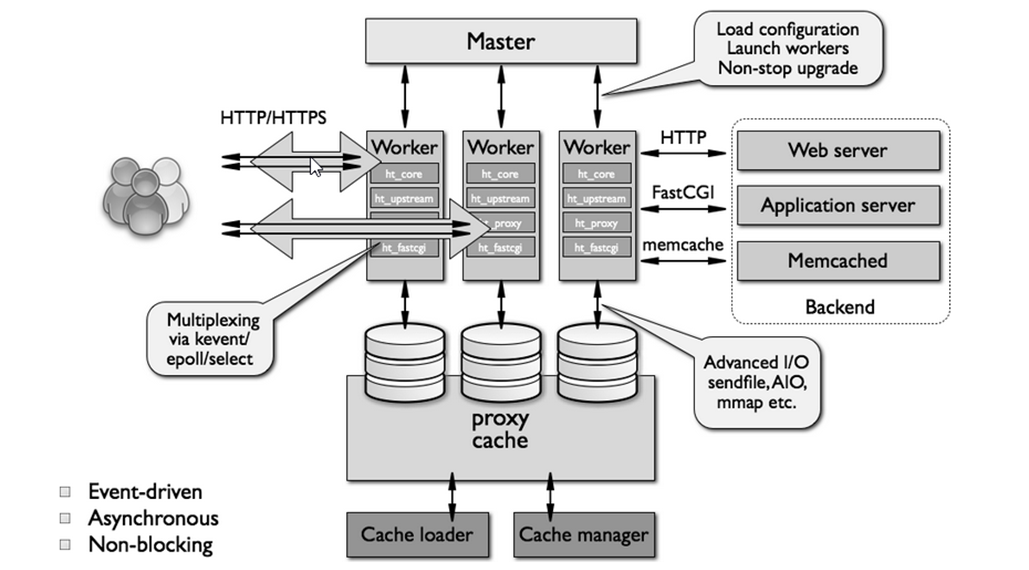
\includegraphics[scale=1]{figuras/nginx-how-it-works} 
	\caption{Modelo de funcionamento do Nginx.}
	\label{fig:nginx-comofunciona}
\end{figure}

O Nginx é utilizado por vários sítios de grande tráfego como Netflix, GitHub, 
Pinterest, dentre outros.

\section{ApacheBench}
O ApacheBench foi criado em 1.996 por Adam Twiss e, posteriormente doado ao 
Apache \textit{Group}. Originalmente, a ferramenta foi desenvolvida para 
verificar o desempenho em servidores HTTP Apache, mas hoje é utilizada para 
fazer testes de desempenho em  praticamente qualquer servidor HTTP.

\section{FastCGI}

De acordo com \cite{fastcgi} FastCGI é uma interface para servidores 
\textit{web} rápida, aberta e segura, que resolve os problemas de desempenho 
herdados do CGI, sem introduzir \textit{overhead} e complexidade de APIs 
proprietárias.

\subsection{\textit{Common Gateway Interface}}

A interface de fato de aplicações em servidores \textit{web} é o CGI, 
implementado pela primeira vez nos servidores da NCSA. O CGI tem muitos 
benefícios:

\begin{itemize}
	\item Simplicidade: é fácil de entender;
	\item Independente de linguagem: Aplicações em CGI podem ser escritas em quase todas a linguagens;
	\item Isolamento do processo: Como os processos são executados 
	separadamente, aplicações com problema não param ou acessam o estado 
	interno do servidor \textit{web};
	\item Padrão aberto: CGI já foi implementado em praticamente todos os 
	servidores;
	\item Independência de arquitetura: O CGI não é ligado a uma arquitetura de computador em particular.
\end{itemize}

CGI tem alguns inconvenientes significantes, sendo o principal problema  o 
desempenho: como um novo processo é criado para cada requisição e descartada 
quando a requisição acaba, a eficiência é baixa.

\subsection{Servidor de API}

Em resposta ao problema de desempenho do CGI, várias empresas desenvolveram 
API's para os seus servidores.

Aplicações conectadas em um servidor de API pode ser significativamente mais 
rápido do que programas desenvolvidos em CGI. O problema da inicialização do 
CGI é melhorada, pois a aplicação é executada no processo do servidor e 
persiste pelas requisições. As API's dos servidores \textit{web} também 
oferecem funcionalidades adicionais comparadas com o CGI. O desenvolvedor pode 
criar extensões que permitem realizar controle de acesso, pegar um acesso dos 
aquivos de registro (\textit{log}) do servidor e, se conectar a outros estágios 
do processamento de uma requisição do servidor. No entanto, API's sacrificam 
todos os benefícios do GCI. São eles:

\begin{itemize}
	\item Complexidade: API's de empresas introduzem uma curva de aprendizado, 
	custos de implementação e manutenção maiores;
	\item Dependência de linguagem: as aplicações devem ser escritas na 
	linguagem de programação suportada pela API;
	\item Não há isolamento de processos: como o processo é executado dentro do 
	endereço de memória do servidor, aplicações com problemas podem corromper o 
	núcleo do servidor, comprometer a segurança e problemas no núcleo do 
	servidor podem corromper as aplicações;
	\item Proprietário: Codificar a aplicação para uma determinada API força o desenvolvedor a utilizar aquele servidor em particular;
	\item Arquiteturas de computador iguais: As aplicações devem usar a mesma 
	arquitetura do servidor \textit{web}.
\end{itemize}

\subsection{FastCGI}

A interface do FastCGI combina os melhores aspectos do CGI e das API's 
proprietárias. Assim como o CGI, o FastCGI executa os processos de forma 
separada e isolada. As vantagens do FastCGI incluem:

\begin{itemize}
	\item Desempenho: Os processos do FastCGI são persistentes, sendo 
	reutilizados para manipular várias requisições, resolvendo o problema da 
	criação de novos processos para cada requisição;
	\item Simplicidade com fácil migração do CGI: a biblioteca de aplicação do FastCGI simplifica a migração de aplicações existentes feitas usando CGI. Aplicações feitas utilizando a biblioteca de aplicações do FastCGI podem ser executadas como programa CGI;
	\item Independência de linguagem: Assim como o CGI, as aplicações FastCGI 
	podem ser escritas em qualquer linguagem;
	\item Isolamento de processos: Uma aplicação com problemas não pode 
	corromper o núcleo do servidor ou de outra aplicação.
	\item Independência de arquitetura: O FastCGI não é ligado a uma arquitetura de computador em particular. Qualquer servidor \textit{web} pode implementar a interface do FastCGI;
	\item Suporte à computação distribuída: FastCGI provê a habilidade de 
	executar aplicações remotamente, o que é útil para distribuir carga e 
	gerenciar sítios da \textit{web} externos.
\end{itemize}

\section{HTML}

De acordo com o \citeonline{w3chtml} a Web é baseada em 3 pilares:

\begin{itemize}
	\item Um esquema de nomes para localização de fontes de informação na Web a 
	URI 
	(\textit{Uniform Resource Identifier});
	\item Um Protocolo de acesso para acessar estas fontes, hoje o HTTP;
	\item Uma linguagem de Hipertexto, para a fácil navegação entre as fontes 
	de informação: o HTML.
\end{itemize}

\subsection{Hipertexto}

HTML é a abreviação para \textit{Hypertext Markup Language} - Linguagem de 
Marcação de Hipertexto. Em resumo, HTML é uma linguagem para publicação de 
conteúdo (texto, imagem, vídeo, áudio e etc) na \textit{web}.

HTML é baseado no conceito de Hipertexto. Hipertextos são conjuntos de 
elementos – ou nós – ligados por conexões. Estes elementos podem ser palavras, 
imagens, vídeos, áudio, documentos etc.. Estes elementos conectados formam uma 
grande rede de informação que não estão conectados linearmente como se fossem 
textos de um livro, onde um assunto é ligado ao outro seguidamente. A conexão 
feita em um hipertexto é algo imprevisível que permite a comunicação de dados, 
organizando conhecimentos e guardando informações relacionadas.

Para distribuir informação de maneira global, é necessário haver uma linguagem 
que seja entendida universalmente por diversos meios de acesso. O HTML se 
propõe a ser esta linguagem. Desenvolvido originalmente por Tim Berners-Lee o 
HTML ganhou popularidade quando o \textit{Mosaic - browser}, desenvolvido por 
Marc Andreessen na década de 1990, ganhou força. A partir de então, 
desenvolvedores e fabricantes de navegadores passaram a utilizar o HTML como 
base, compartilhando sas mesmas convenções.

\subsection{HTML}

Entre 1993 e 1995, o HTML ganhou as versões HTML+, HTML2.0 e HTML3.0, onde 
foram propostas diversas mudanças para enriquecer as possibilidades da 
linguagem. Contudo, até 1.995 o HTML ainda não era tratado como um padrão. 
Apenas em 1997, o grupo de trabalho W3C, responsável por manter o padrão do 
código, trabalhou na versão 3.2 da linguagem, fazendo com que ela fosse tratada 
como padrão.

Desde o começo o HTML foi criado para ser uma linguagem independente de 
plataformas, navegadores e outros meios de acesso. Interoperabilidade significa 
menos custo. O desenvolvedor cria apenas um código HTML e este código pode ser 
lido por diversos dispositivos ao invés de versões diferentes para cada 
dispositivo. Dessa forma, evita-se que a \textit{Web} seja desenvolvida em uma 
base proprietária, com formatos incompatíveis e de forma limitada. Por esses 
motivos o HTML foi desenvolvido para que essa barreira fosse ultrapassada, 
fazendo com que a informação publicada por meio deste código fosse acessível 
por dispositivos e outros meios com características diferentes, não importando 
o tamanho da tela, resolução, variação de cor, dentre outros. O HTML deve ser 
entendido universalmente, dando a possibilidade para a reutilização dessa 
informação de acordo com as limitações de cada meio de acesso.

\section{PHP}
PHP (acrônimo para preprocessador de hipertexto) é uma linguagem de programação 
de código aberto, interpretada, de propósito geral, de tipagem dinâmica e 
fraca, procedural, reflexiva, orientada a objetos e funcional; criada em 1.995 
por Rasmus Lerdorf. A linguagem é melhor utilizada para criação de sistemas 
baseados na \textit{web}, já que pode ser inserida diretamente em códigos 
HTML.

De acordo com \citeonline{phpwhatcando}, o PHP pode realizar qualquer tipo de 
atividade computacional. Tem como foco executar tarefas do lado do servidor, 
realizando qualquer tarefa que uma aplicação feita em CGI pode fazer tais como: 
coletar dados de um formulário, gerar páginas com conteúdo dinâmico ou enviar e 
recebe \textit{cookies}. Existem três áreas onde o PHP é mais utilizado:

\begin{itemize}
	\item \textit{Script} do lado do servidor: é a forma mais tradicional e o 
	principal foco do PHP;
	\item \textit{Script} de linha de comando: é uma forma de utilizar o PHP 
	sem um servidor \textit{web} ou navegador de internet. Esse forma de uso é 
	ideal para rotinas programadas executadas no sistema operacional. Pode ser 
	usada também para tarefas de processamento de texto;
	\item Aplicações para \textit{Desktop}: PHP provavelmente não é a melhor 
	linguagem para desenvolver aplicações com interface gráfica para 
	computadores de mesa, mais pode ser utilizada para criação de aplicações do 
	lado do cliente utilizando o a extensão PHP-GTK, não distribuída de forma 
	oficial pelos mantenedores da linguagem PHP.
\end{itemize}

Para que o PHP funcione é preciso três coisas: Um interpretador, um servidor 
\textit{web} e um navegador de \textit{internet}. Pode ser utilizado em 
praticamente todos os sistemas operacionais e ser executado em qualquer 
servidor \textit{web} que utilize a extensão FastCGI PHP.\\
Com o PHP, o desenvolvedor não fica limitado a somente gerar páginas HTML, 
incluindo as habilidades de entregar imagens e arquivos em geral, geração de 
páginas em XHTML e qualquer outro arquivo XML e servindo como \textit{cache} no 
servidor para o conteúdo gerado dinamicamente.\\
Uma das funcionalidades mais importantes do PHP é o suporte a uma grande 
variedade de bancos de dados. Desenvolver páginas que utilizam base de dados é 
simples, desde que se use uma extensão para base de dados presente na 
linguagem, uma camada de abstração, como por exemplo o PDO, ou conectar a 
qualquer base de dados que suporte o padrão ODBC.\\
O PHP tem ferramentas de processamento de texto úteis, incluindo analisador de 
expressões regulares compatível com a linguagem de programação Perl, além de 
várias outras extensões e ferramentas para analisar e acessar documentos no 
formato XML.

\subsection{PHP-FPM}
O PHP-FPM (\textit{(FastCGI Process Manager}) é uma implementação alternativa do PHP FastCGI com algumas funcionalidades úteis, principalmente, para sítios com grande acesso. Essas funcionalidade incluem:

\begin{itemize}
	\item Gerenciamento avançado de processos;
	\item Habilidade para iniciar processos com diferentes usuários, grupos e ambientes, escutando portas diferentes e usando diferentes arquivos de configuração;
	\item Registro (\textit{log}) de atividades nas saídas padrão de texto 
	(stdout) e de erros (stderr) do sistema operacional;
	\item Reinicialização emergencial em caso de destruição acidental da memória cache;
\end{itemize}

\section{PostgreSQL}

De acordo com \citeonline{postgresql} PostgreSQL é um sistema gerenciador de 
banco de dados objeto-relacional que tem sido desenvolvido de várias formas 
desde 1.977. Começou como um projeto chamado Ingres na \textit{University of 
California} em Berkeley, Estados Unidos. O Ingres foi, posteriormente, 
desenvolvido comercialmente pela empresa Relational Technologies.

Em 1.986 uma outra equipe chefiada por Michael Stonebraker continuou o 
desenvolvimento do código do Ingres para criar um sistema de banco de dados 
usando o paradigma objeto-relacional chamado Postgres. Em 1.996, o Postgres foi 
renomeado para PostgreSQL.

O PostgreSQL é considerado por muitos o melhor SGBD de código aberto do mundo, 
provendo várias funcionalidades que, normalmente, são vistas somente em 
produtos comerciais desenvolvidos para grande empresas.

\section{Miolo \textit{framework}}

O Miolo é um \textit{framework} para criação de sistemas de informação 
acessíveis via \textit{web} escrito em PHP. O Miolo utiliza \textit{scripts} 
javascript e conceitos de programação orientada a objetos, gerando páginas HTML 
e arquivos PDF. Com um projeto modular, baseado em componentes, e uma 
arquitetura em camadas, o Miolo atua como ``\textit{kernel}'' de todos os 
sistemas criados. Favorecendo a reutilização, os vários sistemas podem ser 
facilmente integrados, funcionando como módulos de um sistema mais complexo. 
Além de proporcionar as funcionalidades para o desenvolvimento de sistemas, o 
Miolo também define uma metodologia de codificação para que os resultados 
esperados sejam obtidos de forma simples e rápida.

Os sistemas desenvolvidos com o Miolo seguem algumas regras básicas que devem 
ser conhecidas, como as definições de classes/\textit{forms}/\textit{handlers} 
dos módulos, definição dos arquivos de configuração (localização dos programas, 
componentes, bancos de dados, temas, etc.), o ciclo de vida de execução de uma 
requisição do cliente, além das principais classes, métodos e controles. 
Algumas das principais funções implementadas pelo framework são:

\begin{itemize}
	\item Controles de interface com o usuário, escritos em PHP e renderizados 
	em HTML;
	\item Autenticação de usuários;
	\item Controle de permissão de acesso;
	\item Camada de abstração para acesso a bancos de dados;
	\item Camada de persistência transparente de objetos;
	\item Gerenciamento de sessões e estado;
	\item Validação de entrada em formulários;
	\item Customização de \textit{layout} e temas usando CSS;
	\item Geração de arquivos em PDF;
\end{itemize}


% ---
% Metodologia
% ---
\chapter{Metodologia}\label{metodologia}

Para comparar o desempenho do APACHE e do Nginx, foram realizados testes usando a ferramenta ApacheBench.\\

O ApacheBench é uma ferramenta para ser utilizada em linha de comando. Para invocar a ferramenta escreve-se o comando “ab” no terminal. A ferramenta aceita como parâmetros, entre outros, a quantidade de requisições que serão feitas e quantas requisições serão feitas de forma simultânea, além URL da \'{a}gina que ser\'{a} requisitada. O comando de uma forma genérica fica assim:\\
\begin{verbatim}
ab -n numero_de_requisições -c requisições_simultâneas endereço_do_servidor
\end{verbatim}
Como visto, o parâmetro “-n” indica a quantidade total de requisições serão feitas no teste e o parâmetro “-c” indica a quantidade de requisições serão feitas de forma simultânea.\\

Para comparar os desempenhos dos dois servidores HTTP, foram realizados teste com quantidade de requisições entre 1.000 (mil) e 15.000 (quinze mil) pulando de mil em mil e com somente uma requisição concorrente e com 10\%, 20\%, 40\% e 80\% de concorrência de acordo com a quantidade de requisições. Esses números foram estimados tendo em vista a quantidade atual de usuário do SIGA e a quantidade de usuário que poderá ter no futuro.\\

Então para cada servidor HTTP, foram feitos 75 testes listados abaixo:\\

\begin{table}[htb]
\ABNTEXfontereduzida
\caption[Requisições Totais e Requisições Concorrentes]{Requisições Totais e Requisições Concorrentes}
\label{tab-nivinv}
\begin{tabular}{|>{\bfseries}c|c|c|c|c|c|}
\hline
\multirow{2}{*}{Requisições Totais} & \multicolumn{5}{c|}{\textbf{Requisições Concorrentes}} \\ \cline{2-6}
& 1 & 10\% & 20\% & 40\% & 80\% \\ \hline
1000	 & 1 & 100 & 200 & 400 & 800 \\ \hline
2000 & 1 & 200 & 400 & 800 & 1600 \\ \hline
3000 & 1 & 300 & 600 & 1200 & 2400 \\ \hline
4000	 & 1 & 400 & 800 & 1600 & 3200 \\ \hline
5000 & 1 & 500 & 1000 & 2000 & 4000 \\ \hline
6000 & 1 & 600 & 1200 & 2400 & 4800 \\ \hline
7000 & 1	 & 700 & 1400 & 2800 & 5600 \\ \hline
8000 & 1 & 800 & 1600 & 3200 & 6400 \\ \hline
9000 & 1 & 900 & 1800 & 3600 & 7200 \\ \hline
10000 & 1 & 1000 & 2000 & 4000 & 8000 \\ \hline
11000 & 1 & 1100 & 2200 & 4400 & 8800 \\ \hline
12000 & 1 & 1200 & 2400 & 4800 & 9600 \\ \hline
13000 & 1 & 1300 & 2600 & 5200 & 10400 \\ \hline
14000 & 1 & 1400 & 2800 & 5600 & 11200 \\ \hline
15000 & 1 & 1500 & 3000 & 6000 & 12000 \\ \hline

\end{tabular}
\legend{Quantidade de Requisições e Requisições Concorrentes}
\end{table}
 
Para cada teste realizado os seguintes dados foram obtidos a partir da resposta do servidor HTTP para o ApacheBench:

\begin{itemize}
\item Tempo total do teste em segundos;
\item Total de dados transferido em bytes;
\item Total de texto em HTML transferido em bytes;
\item Número de requisições atendidas por segundo;
\item Tempo médio por requisição em milissegundos;
\item Tempo médio por requisição entre as requisições concorrentes em milissegundos;
\item Taxa de transferência em Quilo Bytes por segundo;
\item Porcentagem das requisições servidas em um período de tempo, tempo em milissegundos.
\end{itemize}


% ---
% Ambiente de Testes
% ---
\section{Ambiente de testes}

Para fazer os teste da forma mais neutra possível, foram criadas duas máquinas virtuais usando o software de virtualização VirtualBox na sua versão 3.4.10.\\
Todos os programas utilizados nos ambientes de teste foram instalados pelo gerenciador de pacotes nativo da distribuição Linux Debian \textit{aptitude} e disponíveis nos repositórios oficiais do Debian, exceto o SGBD PostgreSQL que foi instalado usando o \textit{aptitude} porém através do repositório oficial do PostgreSQL para o Linux Debian 7 pois nos repositórios do Debian não havia disponível a versão mais recente e utilizada pelo banco de dados do SIGA.

\subsection{Computador hospedeiro}
O computador onde foram instaladas as máquinas virtuais possui a seguinte 
configuração:
\begin{itemize}
	\item \textbf{Tipo}: Computador portátil (\textit{Notebook})
	\item \textbf{Processador}: Intel Core i5-3337U
	\item \textbf{Frequência do Processador}: 1,8 Giga Hertz
	\item \textbf{Tamanho da Memória Principal (RAM)}: 8 Giga Bytes;
	\item \textbf{Tamanho da Memória Secundária (HD)}: 1 Tera Bytes;
	\item \textbf{Quantidade de núcleos disponível para processamento}: 4 
	núcleos.
\end{itemize}

\subsection{Configurações comuns às duas máquinas virtuais}
 Ambas máquinas virtuais tinhas as configurações rigorosamente iguais. São elas:
\begin{itemize}
\item \textbf{Sistema Operacional}: Linux Debian 7 “Wheezy” 64 bits mais atualizado;
\item \textbf{Sistema Gerenciador de Banco de Dados}: PostgreSQL na versão 9.3.5
\item \textbf{Tamanho da Memória Principal (RAM)}: 2.048 Mega Bytes;
\item \textbf{Tamanho da Memória Secundária (HD)}: 30 Giga Bytes;
\item \textbf{Quantidade de núcleos disponível para processamento}: 1 núcleo.
\end{itemize}

\subsection{Máquina virtual Apache}
Na máquina virtual destinada aos testes com o servidor HTTP Apache, os programas utilizados foram:
\begin{itemize}
\item Apache HTTP Server na versão 2.2.22;
\item libapache2-mod-php5 na versão 5.4.4;
\item php5-common na versão 5.4.4.
\end{itemize}

\subsection{Máquina virtual Nginx}
Na maquina virtual destinada aos testes com o servidor HTTP Nginx, os programas utilizados foram:

\begin{itemize}
\item Servidor HTTP Nginx na versão 1.2.1;
\item php5-fpm na versão 5.4.4;
\item php5-common na versão 5.4.4.
\end{itemize}



% ----------------------------------------------------------
% ELEMENTOS PÓS-TEXTUAIS
% ----------------------------------------------------------
\postextual
% ----------------------------------------------------------

% ----------------------------------------------------------
% Referências bibliográficas
% ----------------------------------------------------------
\bibliography{bibliografia}

\end{document}

